\documentclass[es,apuntes]{uah}

\tema{1}
\titulo{Teoría de la información}{Lesson title}

\begin{document}

\titulacion{Optativa GIEC y GIT}
\departamento{Teoría de la Señal y Comunicaciones}
\asignatura{Comunicaciones Digitales}{}
\curso{2022/2023} 

\maketitle


%%%%%%%%%%%%%%%%%%%%%%%
\section{Medida de la información}
%%%%%%%%%%%%%%%%%%%%%%%

Cuando nos referimos a un sistema de comunicaciones estamos acostumbrados a decir que tiene como objetivo la transmisión de información entre dos puntos. Ahora bien, cabe preguntarse ¿qué entendemos por información? 
Podemos modelar la salida de cualquier fuente (voz, vídeo, datos, etc.) como un proceso aleatorio. Para el caso de procesos aleatorios discretos, estacionarios y sin memoria, se puede definir la {\bf cantidad de información} como:

\begin{displaymath}
	I = -log_2(p_k)
\end{displaymath}

donde $p_k$ representa la probabilidad de aparición de cada uno de los símbolos de la fuente. Si consideramos el caso de que uno de los símbolos tenga $p_k=1$, es decir, que no exista ningún tipo de incertidumbre, sino que sepamos perfectamente qué símbolo se va a transmitir en todo momento, podemos ver que la información de este tipo de fuente es $0$. Para cualquier otro caso la información tomará un valor positivo, y será tanto mayor cuanto menor sea la probabilidad de ocurrencia del símbolo.

Si cualculamos la media estadística de los valores de información de una fuente para cada uno de los símbolos obtenemos lo que se denomina {\bf entropía} de la fuente:

\begin{equation}
	H = - \sum_{k=1}^{N}p_k \cdot  log_2(p_k)
\end{equation}

Habitualmente la entropía se mide en bits (siempre que se use el logaritmo con base 2. Si se usase un logaritmo neperiano, la unidad serían \emph{nats}), y nos da una idea de cuántos bits por símbolo como mínimo se necesitan para codificar una determinada fuente de forma exacta. Visto desde otro punto de vista, también podemos entender la entropía como una medida de la incertidumbre sobre el valor concreto que tomará una variable aleatoria (en nuestro caso, los símbolos transmitidos por la fuente). Igual que decíamos antes, si la variable toma siempre el mismo valor (es decir, que haya un $p_k$ con $p_k=1$), no tenemos ninguna incertidumbre sobre el valor que tomará el símbolo transmitido, y por tanto la entropía será cero.


%%%%%%%%%%%%%%%%%%%%%%%
\section{Codificación de fuente}
%%%%%%%%%%%%%%%%%%%%%%%

La codificación de fuente, o codificación sin ruido, se refiere al conjunto de técnicas que permiten reducir el número de bits necesarios para representar la salida de una fuente sin perder la posibilidad de reconstrucción perfecta. En general, un codificador fuente utilizará palabras binarias con menos bits para aquellos símbolos más probables, y más bits para las menos probables. Un ejemplo de código de este tipo es el código Morse, que por ejemplo utiliza un '.' para la letra \emph{E}, muy probable en general, y el código '--.-' para la \emph{Q}, mucho menos probable. 

El teorema de codificación de fuente de Shannon nos dice que, para reconstruir perfectamente una fuente, {\bf es posible utilizar un código con un número de bits por símbolo nunca inferior a la entropía de la fuente}.

En la práctica existen distintos algoritmos de codificación de fuente, pero nosotros vamos a centrarnos en los denominados códigos prefijo (\emph{prefix codes}), que se caracterizan porque ninguna palabra código es \emph{prefijo} de otra palabra código. La ventaja de esta aproximación es que podemos transmitir los códigos binarios de los símbolos uno tras otro, sin ninguna separación, y el decodificador será capaz de reconstruir el mensaje sin ninguna ambigüedad. Un caso particular de códigos prefijo, aunque en muchos casos se les confunde, son los códigos Huffman, creados por David Huffmann en 1951 cuando preparaba un trabajo para una asignatura de doctorado en el MIT, donde estudiaba.


\subsection{Codificación Huffman}

La idea que hay detrás de los {\bf códigos Huffman} es muy sencilla: como decíamos, se asignan palabras con más bits a aquellos símbolos de la fuente menos probables, y palabras más cortas a los símbolos más probables. Para hacerlo, empezamos uniendo los dos símbolos menos probables para generar un nuevo símbolo cuya probabilidad de aparición será la suma de las dos probabilidades anteriores. Este proceso se repite hasta que sólo quede un símbolo, y de esta forma se va generando un árbol. 


Ahora, empezando desde la raíz del árbol, vamos asignando \bits{0}s y \bits{1}s a cualesquiera dos ramas que surjan del mismo nodo, y de esta manera se irá creando el código. 

Vamos a verlo con un ejemplo muy sencillo. Imaginemos una fuente con un alfabeto de nueve símbolos con las siguientes probabilidades: 

\begin{displaymath}
\mathbf{p} = (0.2, 0.15, 0.13, 0.12, 0.1, 0.09, 0.08, 0.07, 0.06)
\end{displaymath}

En la primera iteración, agrupamos los dos símbolos menos probables, generando un nuevo símbolo con probabilidad $0.07 + 0.06 = 0.13$. Ordenamos el nuevo vector de probabilidades, obteniendo ahora:

\begin{displaymath}
	\mathbf{p} = (0.08, 0.09, 0.1, 0.12, 0.13, 0.13, 0.15, 0.2)
\end{displaymath}

Repetimos el proceso, agrupando los dos símbolos menos probables, obteniendo un nuevo símbolo con probabilidad $0.08 + 0.09 = 0.17$, y por tanto un nuevo vector de probabilidades que, tras ordenarlo, queda:

\begin{displaymath}
	\mathbf{p} = (0.1, 0.12, 0.13, 0.13, 0.15, 0.17, 0.2)
\end{displaymath}

Si seguimos iterando este algoritmo, en los siguientes pasos iremos obteniendo los siguientes vectores de probabilidades de error:

\begin{displaymath}
	\mathbf{p} = (0.13, 0.13, 0.15, 0.17, 0.2, 0.22)
\end{displaymath}

\begin{displaymath}
	\mathbf{p} = (0.15, 0.17, 0.2, 0.22, 0.26)
\end{displaymath}

\begin{displaymath}
	\mathbf{p} = (0.2, 0.22, 0.26, 0.32)
\end{displaymath}

\begin{displaymath}
	\mathbf{p} = (0.26, 0.32, 0.42)
\end{displaymath}

\begin{displaymath}
	\mathbf{p} = (0.42, 0.58)
\end{displaymath}

Ahora viene el momento de ir retrocediendo. Empezamos asignando un \bits{0} al símbolo con probabilidad $0.42$, y un \bits{1} al otro. En el siguiente paso, el símbolo con probabilidad $0.58$ se descompone en dos, con probabilidades $0.26$ y $0.32$. Así que al \bits{1} de antes, le añadimos un \bits{0} en el primer caso, y un \bits{1} en el segundo. Tenemos por tanto que el símbolo con probabilidad $0.26$ se codifica con un \bits{10}, el de probabilidad $0.32$ con \bits{11} y el de probabilidad $0.42$ con \bits{0}.

Igual que antes, vamos repitiendo este proceso hasta llegar a los 9 símbolos originales, obteniéndose este resultado:

\begin{center}
\begin{tabular}{ c c c}
	Símbolo & Probabilidad & Código\\
	\hline
	$s_1$ & $0.2$	& \bits{00} \\
	$s_2$ & $0.15$	& \bits{110} \\
	$s_3$ & $0.13$  & \bits{101} \\
	$s_4$ & $0.12$	& \bits{011} \\
	$s_5$ & $0.1$	& \bits{010} \\
	$s_6$ & $0.09$	& \bits{1111} \\
	$s_7$ & $0.08$	& \bits{1110} \\
	$s_8$ & $0.07$	& \bits{1001} \\
	$s_9$ & $0.06$	& \bits{1000} \\
\end{tabular}

\end{center}

Para evaluar la calidad de un código fuente se pueden utilizar distintos parámetros, aunque nosotros nos vamos a fijar sólo en dos: la tasa de compresión y la eficiencia. 

Definimos {\bf longitud media} de un código como la longitud promedio de las palabras del mismo:

\begin{equation}
\bar{L} = \sum_{i=1}^M p_i n_i	
\end{equation}

donde $n_i$ es el número de bits utilizados para codificar el símbolo $i$-ésimo. 

Se puede comprobar de forma muy sencilla que la longitud media de palabra para este código es:

\begin{displaymath}
	\bar{L} = 2\cdot 0.2 + 3 \cdot (0.15 + 0.13 + 0.12 + 0.1) + 4 \cdot (0.09 + 0.08 + 0.07 + 0.06) = 3.1
\end{displaymath}

A partir de la longitud media podemos definir la {\bf tasa de compresión} como la relación de compresión lograda frente a un código de longitud fija:

\begin{equation}
	\Gamma = \frac{\lceil log_2 M \rceil}{\bar{L}}
\end{equation}

Por otro lado, la {\bf eficiencia} de un código mide lo cerca que se encuentra su longitud media del límite teórico dado por la entropía:

\begin{equation}
	\eta = \frac{H(x)}{\bar{L}}
\end{equation}

Lógicamente, según el teorema de Shannon, será imposible obtener valores de la eficiencia superiores a $1$. 

Es posible demostrar que la longitud media de palabra de un código Huffman cumple la siguiente desigualdad:

\begin{equation}
	H \leq \bar{L} \leq H+1
\end{equation}

Y si agrupamos los símbolos en grupos de $K$, en lugar en enviarlos de forma individual, se obtiene que:

\begin{equation}
	H \leq \bar{L} \leq H + \frac{1}{K}
\end{equation}

Es decir, al incrementar el valor de $K$ nos vamos a poder acercar cada vez más al valor de la entropía, aunque a costa, eso sí, de incrementar la complejidad del sistema de forma importante. 

%%%%%%%%%%%%%%%%%%%%%%%%%%%%%
\subsection{Codificación LZW}
%%%%%%%%%%%%%%%%%%%%%%%%%%%%%

Uno de los inconvenientes de los códigos Huffman es que, para generarlos, necesitamos conocer las probabilidades de ocurrencia de cada uno de los símbolos, lo que no siempre es posible, aunque se pueden realizar estimaciones. 

Unos de los códigos más utilizados es el LZW, que surgió como una versión del algoritmo LZ78 desarrollado por Abraham Lempel y Jacob Ziv, y mejorado por Terry Welch (el nombre del algoritmo viene de las iniciales de cada uno de sus creadores). 

Este método de codificación fue el estándar del comando \emph{compress} de Unix durante muchos años, hasta que se dejó de utilizar por algunos problemas de patentes. Asimismo, forma parte del formato de imagen GIF y también se puede utilizar para reducir el tamaño de los archivos TIFF.

En forma de pseudocódigo, podemos escribir el algoritmo de la siguiente forma:

\begin{verbatim}
     CADENA = cadena vacía
     WHILE queden caracteres por codificar DO
          CARACTER = coger el siguiente carácter
          IF CADENA+CARACTER está en el diccionario
               CADENA = CADENA+CARACTER
          ELSE
               código correspondiente a CADENA -> SALIDA
               Añadir CADENA+CARACTER al diccionario
               CADENA = CARACTER
          END
     END
   	 código para CADENA -> SALIDA
\end{verbatim}

Imaginemos que tenemos un diccionario que tiene las siguientes entradas: \\

\begin{tabular}{cc}
Código & Entrada \\
0 & a \\
1 & b \\	
2 & n \\
\end{tabular}
\ \\

Y ahora supongamos que la cadena de entrada al codificador es \emph{banana}. La codificación sería:\\


\begin{tabular}{lcclc}
CADENA & CARACTER  & ¿En el Diccionario? & Al Diccionario & Salida \\
\hline
 	& b & Si &  &  \\
 b & a & No & 3 - ba & 1 \\
 a & n & No & 4 - an & 0 \\
 n & a & No & 5 - na & 2 \\
 a & n & Sí & 		&  \\
 an & a & No & 6 - ana & 4 \\
 a & & & & 0 \\ 	
\end{tabular}

\ \\
Es decir, la señal codificada sería: \texttt{1 0 2 4 0}. \\

\ \\
\ \\

La decodificación, por su parte, se hace de la siguiente forma:

\begin{verbatim}
     CODIGO_1 = Leer primer código del mensaje
     Traducción de CODIGO_1 -> SALIDA
     WHILE queden caracteres por decodificar
          CODIGO_2 = Leer siguiente código
          CADENA = traducción de CODIGO_2
          CADENA -> SALIDA
          CARACTER = Primer carácter de CADENA
          Añadir (Traducción de CODIGO_1)+(CARACTER) al diccionario
          CODIGO_1 = CODIGO_2
     END
\end{verbatim}


\begin{tabular}{lccccc}
CODIGO1 & CODIGO2  & CADENA & CARACTER & Salida & Dicc.\\
\hline
1 &   &   &   & b &\\
1 & 0 & a & a & a & 3 - ba \\
0 & 2 & n & n & n & 4 - an \\
2 & 4 & an & a & an & 5 - na \\
4 & 0 & a & a & a & 6 - ana \\
\end{tabular}

\ \\
Se puede ver que la salida es la misma palabra que había a la entrada y que se ha generado también el mismo diccionario que se generó en el proceso de codificación. 



\section{Canal discreto sin memoria}

En la siguiente figura se puede ver un esquema típico de un sistema de comunicaciones digitales. El canal, tal y como se muestra en la figura, tiene a su entrada la señal analógica producida por el modulador y produce a su salida otra señal analógica consistente en la anterior a la que se le suma ruido aditivo gausiano. Este tipo de canal se denomina {\bf canal gausiano}. 

\begin{center}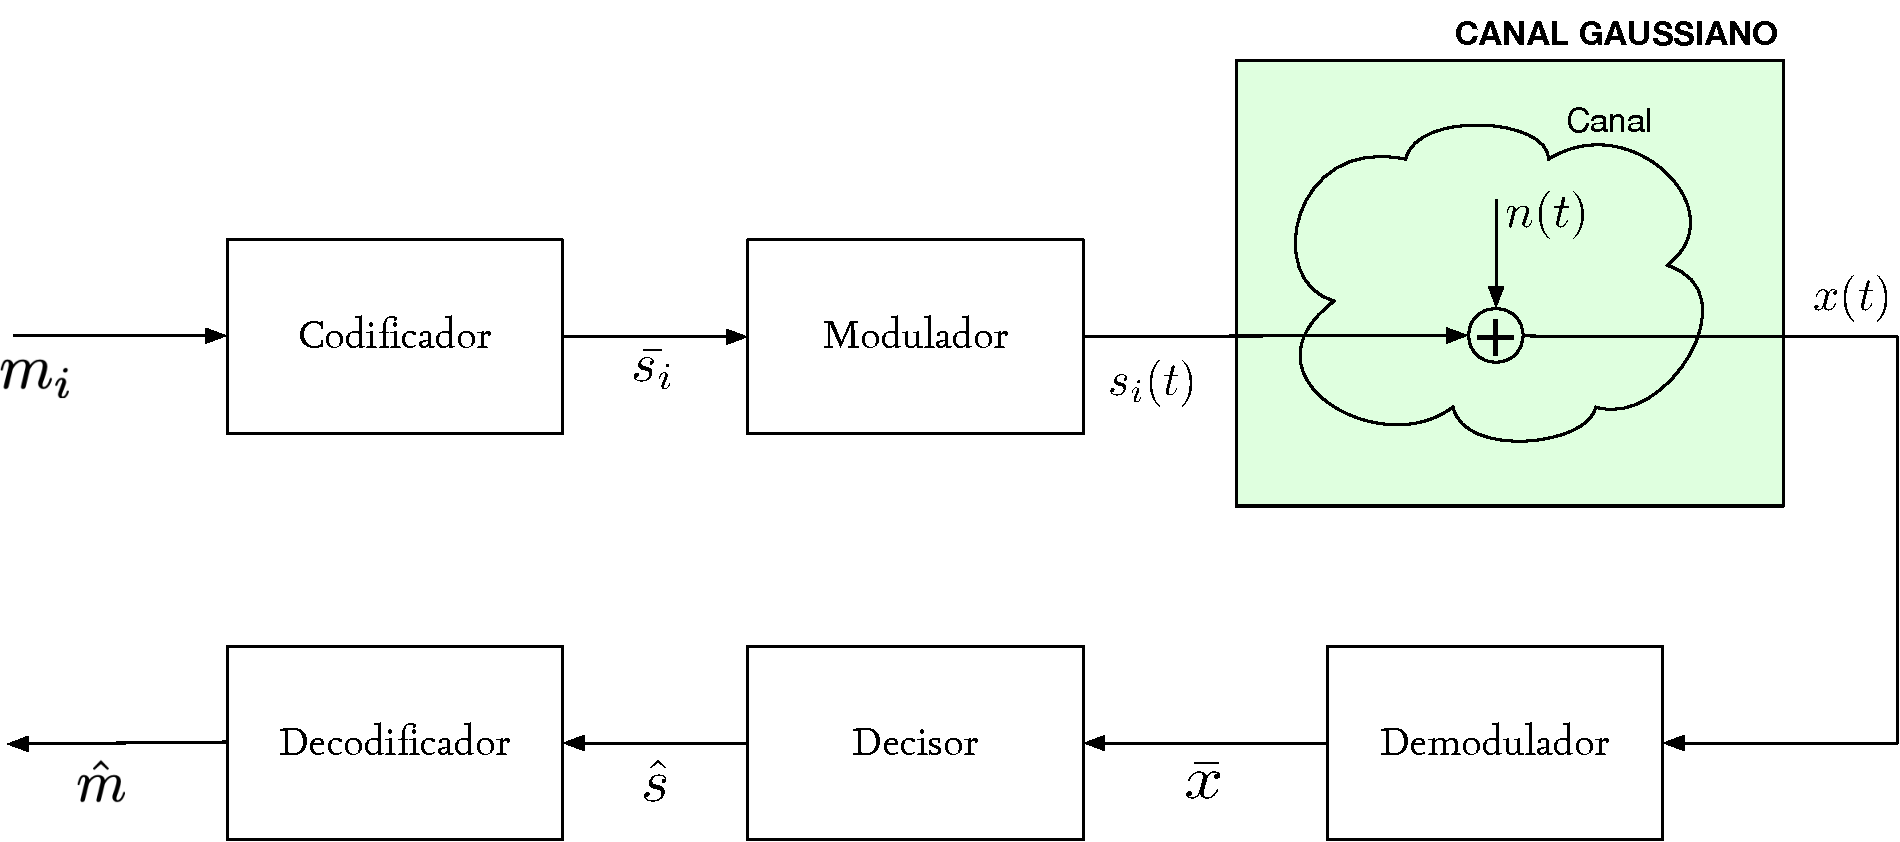
\includegraphics[width=14cm]{../Transparencias/Figuras/Sistema2.pdf}\end{center}

Una alternativa a lo anterior es considerar un canal que tenga a su entrada y salida señales discretas, tal y como se muestra en la siguiente figura:

\begin{center}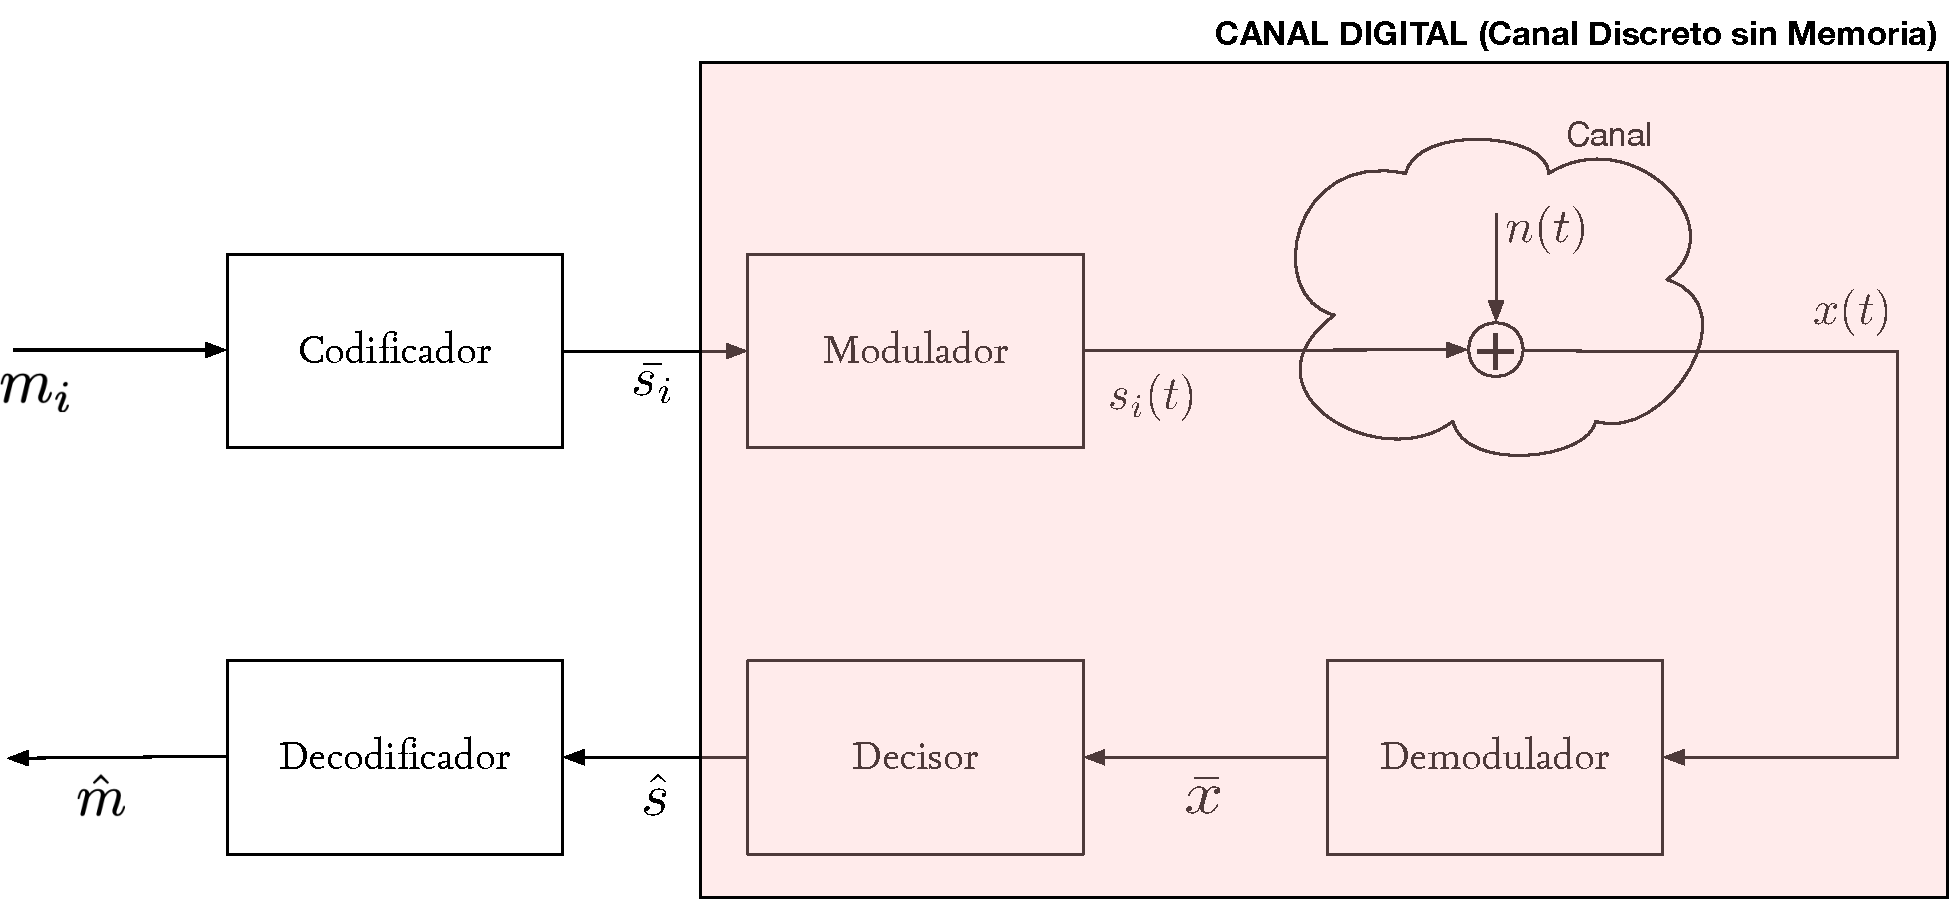
\includegraphics[width=14cm]{../Transparencias/Figuras/Sistema3.pdf}\end{center}

En este caso nos encontramos con lo que se denomina un {\bf canal digital}, que tiene a su entrada un símbolo producido por el codificador, y devuelve otro símbolo que será posteriormente interpretado por el decodificador. El canal digital es un caso particular de lo que se denomina {\bf canal discreto sin memoria}, que relaciona una variable aleatoria $X$ con función de densidad de probabilidad discreta con otra variable aleatoria $Y$, también discreta. La diferencia entre ambas aproximaciones es que el canal discreto equivalente contempla la posibilidad de que los alfabetos de los símbolos a entrada y salida sean distintos. 

Una forma de modelar el funcionamiento de este tipo de canales es mediante una matriz que indique las distintas probabilidades de transición de un símbolo a la entrada a otro a la salida:

\begin{displaymath}
	\mathbf{P} = \left ( \begin{array}{cccc} P_{\hat{S}/S}(\hat{s_1}|s_1) & P_{\hat{S}/S}(\hat{s_2}|s_1) & \cdots &  P_{\hat{S}/S}(\hat{s_N}|s_1) \\ 
	  \vdots & \vdots &  & \vdots \\
	  P_{\hat{S}/S}(\hat{s_1}|s_N) & P_{\hat{S}/S}(\hat{s_2}|s_N) & \cdots &  P_{\hat{S}/S}(\hat{s_N}|s_N) \\ \end{array} \right )
\end{displaymath}

Esta matriz se denomina {\bf matriz de transición} o {\bf matriz de canal}, y cumple la propiedad de que las suma de los elementos de cada fila tiene que ser uno. 

Un caso particular del canal discreto sin memoria en el que el número de símbolos tanto a la entrada como a la salida es dos, es el {\bf canal binario simétrico}. En este caso la matriz de transición viene dada por una expresión como la siguiente:

\begin{displaymath}
	\mathbf{P} = \left ( \begin{array}{cc} 1-p & p \\ p & 1-p \\ \end{array} \right )
\end{displaymath}

donde el valor de $p$ equivale a la probabilidad de error de bit del sistema. 


\section{Entropía condicional e información mútua}

Hemos visto antes que la entropía de una fuente se puede interpretar como la cantidad de incertidumbre que tenemos sobre dicha fuente. Podríamos preguntarnos cuál es la incertidumbre que tenemos sobre los símbolos transmitidos una vez que hemos podido observar los símbolos recibidos. Para conseguir esto se puede extender el concepto de entropía visto antes y definir la entropía condicional, $H(X|Y)$. Por tanto, si $H(X)$ es la incertidumbre de los símbolos transmitidos y $H(X|Y)$ la incertibumbre de los símbolos transmitidos tras observar los símbolos recibidos, la diferencia entre ambas, $H(X) - H(X|Y)$ se puede interpretar como la cantidad de incertidumbre sobre los símbolos transmitidos que somos capaces de resolver gracias a observar los símbolos recibidos. A esta diferencia se le denomina información mútua:

\begin{displaymath}
    I(X,Y)= H(X) - H(X|Y)
\end{displaymath}

Podemos ver dos casos extremos

Visto de otro modo, podemos entender la información mútua entre la entrada y la salida de un canal como la cantidad de información que pasa de la entrada a la salida cuando se utiliza dicho canal. 



\section{Capacidad del canal}
A partir de los conceptos de entropía e información mútua podemos determinar la cantidad máxima de información que se puede transmitir a través de un canal. Si pensamos en la información mútua como la cantidad de información que pasa de la entrada a la salida de un canal, es razonable pensar que la capacidad del canal será el valor máximo que pueda tomar la información mútua entre la entrada y la salida, que en la práctica dependerá no sólo de las características del canal, sino también de la distribución de probabilidades a la entrada. De forma matemática:

\begin{displaymath}
	C = \max_{p(x_i)} I(X,Y)
\end{displaymath}

En general el cálculo de la capacidad del canal es una tarea complicada, pero podemos hacerlo para un caso sencillo como es el del canal binario simétrico que introdujimos antes con símbolos equiprobables a la entrada. En ese caso, es posible comprobar que la capacidad del canal viene dada por la siguiente expresión:

\begin{displaymath}
C = 1 + p log_2 p + (1-p)log_2(1-p) 
\end{displaymath}

siendo $p$ la probabilidad de transición del canal. Podemos pensar en dos casos particulares para entender mejor qué sucede:

\begin{itemize}
\item Si $p=0$, es decir, si el canal no introduce errores, obtenemos que el valor máximo posible de la capacidad del canal , $C=1$ bit. Esto es, el canal puede transmitir un bit de información, que es exactamente la información que hay a la entrada. 
\item Si $p=1/2$, obtenemos el valor mínimo de la capacidad del canal, $C=0$ bits. En este caso el canal no es capaz de transmitir nada de información, y estaríamos hablando de un canal \emph{inútil}. 
\end{itemize}



%\printindex
\end{document}



	
 